\scanpage{18}
\[
(2)\quad\left\{\begin{gathered}
\sigma_0^2=\sigma_1^2=\sigma_\infty^2=1\\
\sigma_0\sigma_1=\deleted{\unsure{l_0\rho}}\inserted{\rho l_0}\qquad
\sigma_1\sigma_\infty=\deleted{\unsure{l_1\rho}}\inserted{\rho l_1}\qquad
\sigma_\infty\sigma_0=\deleted{l_\infty\rho}\inserted{\rho l_\infty}
\end{gathered}\right.
\]
\margin{NB Comme $\sigma_1=\rho\sigma_0\rho^{-1}\ldots$, ces $\leftarrow$ relations s'écrivent aussi
\deleted{\[
\begin{aligned}
l_0&=(\sigma_0\rho)^2\unsure{\sigma_\infty}(\unsure{l_0\sigma_0\sigma_0\rho^{-1}})\\
l_1&=(\sigma_1\rho)^2\unsure{\sigma_1}\qquad&\unsure{l_0}&=\unsure{\rho^{-1}\sigma_0}\\
l_\infty&=(\sigma_\infty\rho)^2\unsure{\sigma_\infty}
\end{aligned}
\]}
\begin{tabular}{|l}
$\begin{aligned}
l_0&=\rho^{-1}\sigma_0\rho\sigma_0\rho^{-1}\\
\deleted{\unsure{\sigma_\infty}}&=\rho^{-1}[\sigma_0,\rho]
\end{aligned}$\\
On a\\
$\begin{aligned}
\deleted{\sigma_0(l_0)=l_1}\\
\deleted{\sigma_0(l_1)=l_0}\\
\deleted{\sigma_0(l_\infty)=\unsure{l_1^{-1}l_0^{-1}}}
\end{aligned}$\\
$\begin{aligned}
\sigma_0(l_0)&=l_\infty^{-1}l_1^{-1}\\
\sigma_0(l_1)&=l_\infty
\end{aligned}$
\end{tabular}
\[
\sigma_0(l_\infty)=l_1
\]}
où $\rho$, au dessus de $\dot\rho$, est défini par le chemin trivial de $P$ à $P$. On a donc
\[
\left\{\begin{aligned}
\rho\sigma_0\rho^{-1}&=\sigma_1\\
\rho\sigma_1\rho^{-1}&=\sigma_\infty\\
\rho\sigma_\infty\rho^{-1}&=\sigma_0
\end{aligned}\right.
\qquad\text{i.e.}\quad
\left\{\begin{aligned}
\rho\sigma_0&=\sigma_1\rho\\
\rho\sigma_1&=\sigma_\infty\rho\\
\rho\sigma_\infty&=\sigma_0\rho
\end{aligned}\right.
\]
On ne voit pas apparaître d'expression de $\rho$ en fonction des $\sigma_0,\sigma_1,\sigma_\infty$ seuls --- \deleted{on voit par contre (utilisant le fait que $l_0,l_1,l_\infty$ avec 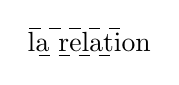
\begin{tikzpicture}[baseline=(relation.base)]
\node[inner sep=0pt,outer sep=0pt] (relation) {la relation};
\draw ([xshift=0.05em,yshift=0.35ex]relation.north west) -- ++(0.42em,0);
\draw ([xshift=0.77em,yshift=0.35ex]relation.north west) -- ++(0.42em,0);
\draw ([xshift=1.49em,yshift=0.35ex]relation.north west) -- ++(0.42em,0);
\draw ([xshift=2.21em,yshift=0.35ex]relation.north west) -- ++(0.42em,0);
\draw ([xshift=2.93em,yshift=0.35ex]relation.north west) -- ++(0.42em,0);
\draw ([xshift=0.40em,yshift=-0.35ex]relation.south west) -- ++(0.42em,0);
\draw ([xshift=1.12em,yshift=-0.35ex]relation.south west) -- ++(0.42em,0);
\draw ([xshift=1.84em,yshift=-0.35ex]relation.south west) -- ++(0.42em,0);
\draw ([xshift=2.56em,yshift=-0.35ex]relation.south west) -- ++(0.42em,0);
\end{tikzpicture} fondamentale (1) est une présentation de $\unsure{\Pi|\pi}$, que \deleted{$\rho$} \inserted{$(\sigma_0\sigma_1)^3$ (p.ex.)} doit s'exprimer en fonction des $l_i$; \unsure{puisque} en outre
\deleted{\[
\rho=l_0l_1l_\infty
\]}
des relations $\sigma_i^2=1$}, il faudra que $\rho$ soit produit de termes $\sigma_i$ \uline{pas deux consécutifs} \deleted{\unsure{distincts|abstrait\textsuperscript{t}}}, \deleted{ou $\sigma_0\sigma_1\sigma_0=$} \inserted{et $\sigma$}
\[
\left\{\begin{aligned}
\dot\sigma_1^2=\dot\sigma_{\unsure{1|0}}^2=\dot\sigma_\infty^2&=1\\
\dot\sigma_0\dot\sigma_1=\dot\sigma_1\dot\sigma_\infty=\dot\sigma_\infty\dot\sigma_0&=\dot\rho\\
\dot\rho^3&=1
\end{aligned}\right.
\quad\text{est une présentation de }\unsure{\mathfrak S_3|\mathcal S_3}\text{),}
\]
\margin{\unsure{comme on voit} \unsure{ils sont} \unsure{\uline{pas} conjugués}}
que le système des relations (1)(2) et enfin
\[
\rho^3=1
\]
est une présentation de l'image inverse de $\unsure{\mathfrak S_3|\mathcal S_3}$ dans $\mathcal E$ (dis dans $\widehat{\mathcal E}$, au pt de vue profini).
\margin{C'est faux, comme on voit en faisant dans les relations $\rho=1$, \unsure{on a le groupe $(\sigma_i)$}}
\mspage{17}
